\documentclass{article}

\usepackage{graphicx}
\usepackage{tikz}
\usepackage{tikzsymbols}
\usetikzlibrary{calc,patterns,shapes.geometric}
\pagestyle{empty}
\usepackage[margin=0pt]{geometry}
\geometry{papersize={14in,12in}}

\def\centerarc[#1](#2)(#3:#4:#5){\draw[#1] ($(#2)+({#5*cos(#3)},{#5*sin(#3)})$) arc (#3:#4:#5);}

\begin{document}
	\begin{figure}
		\centering
		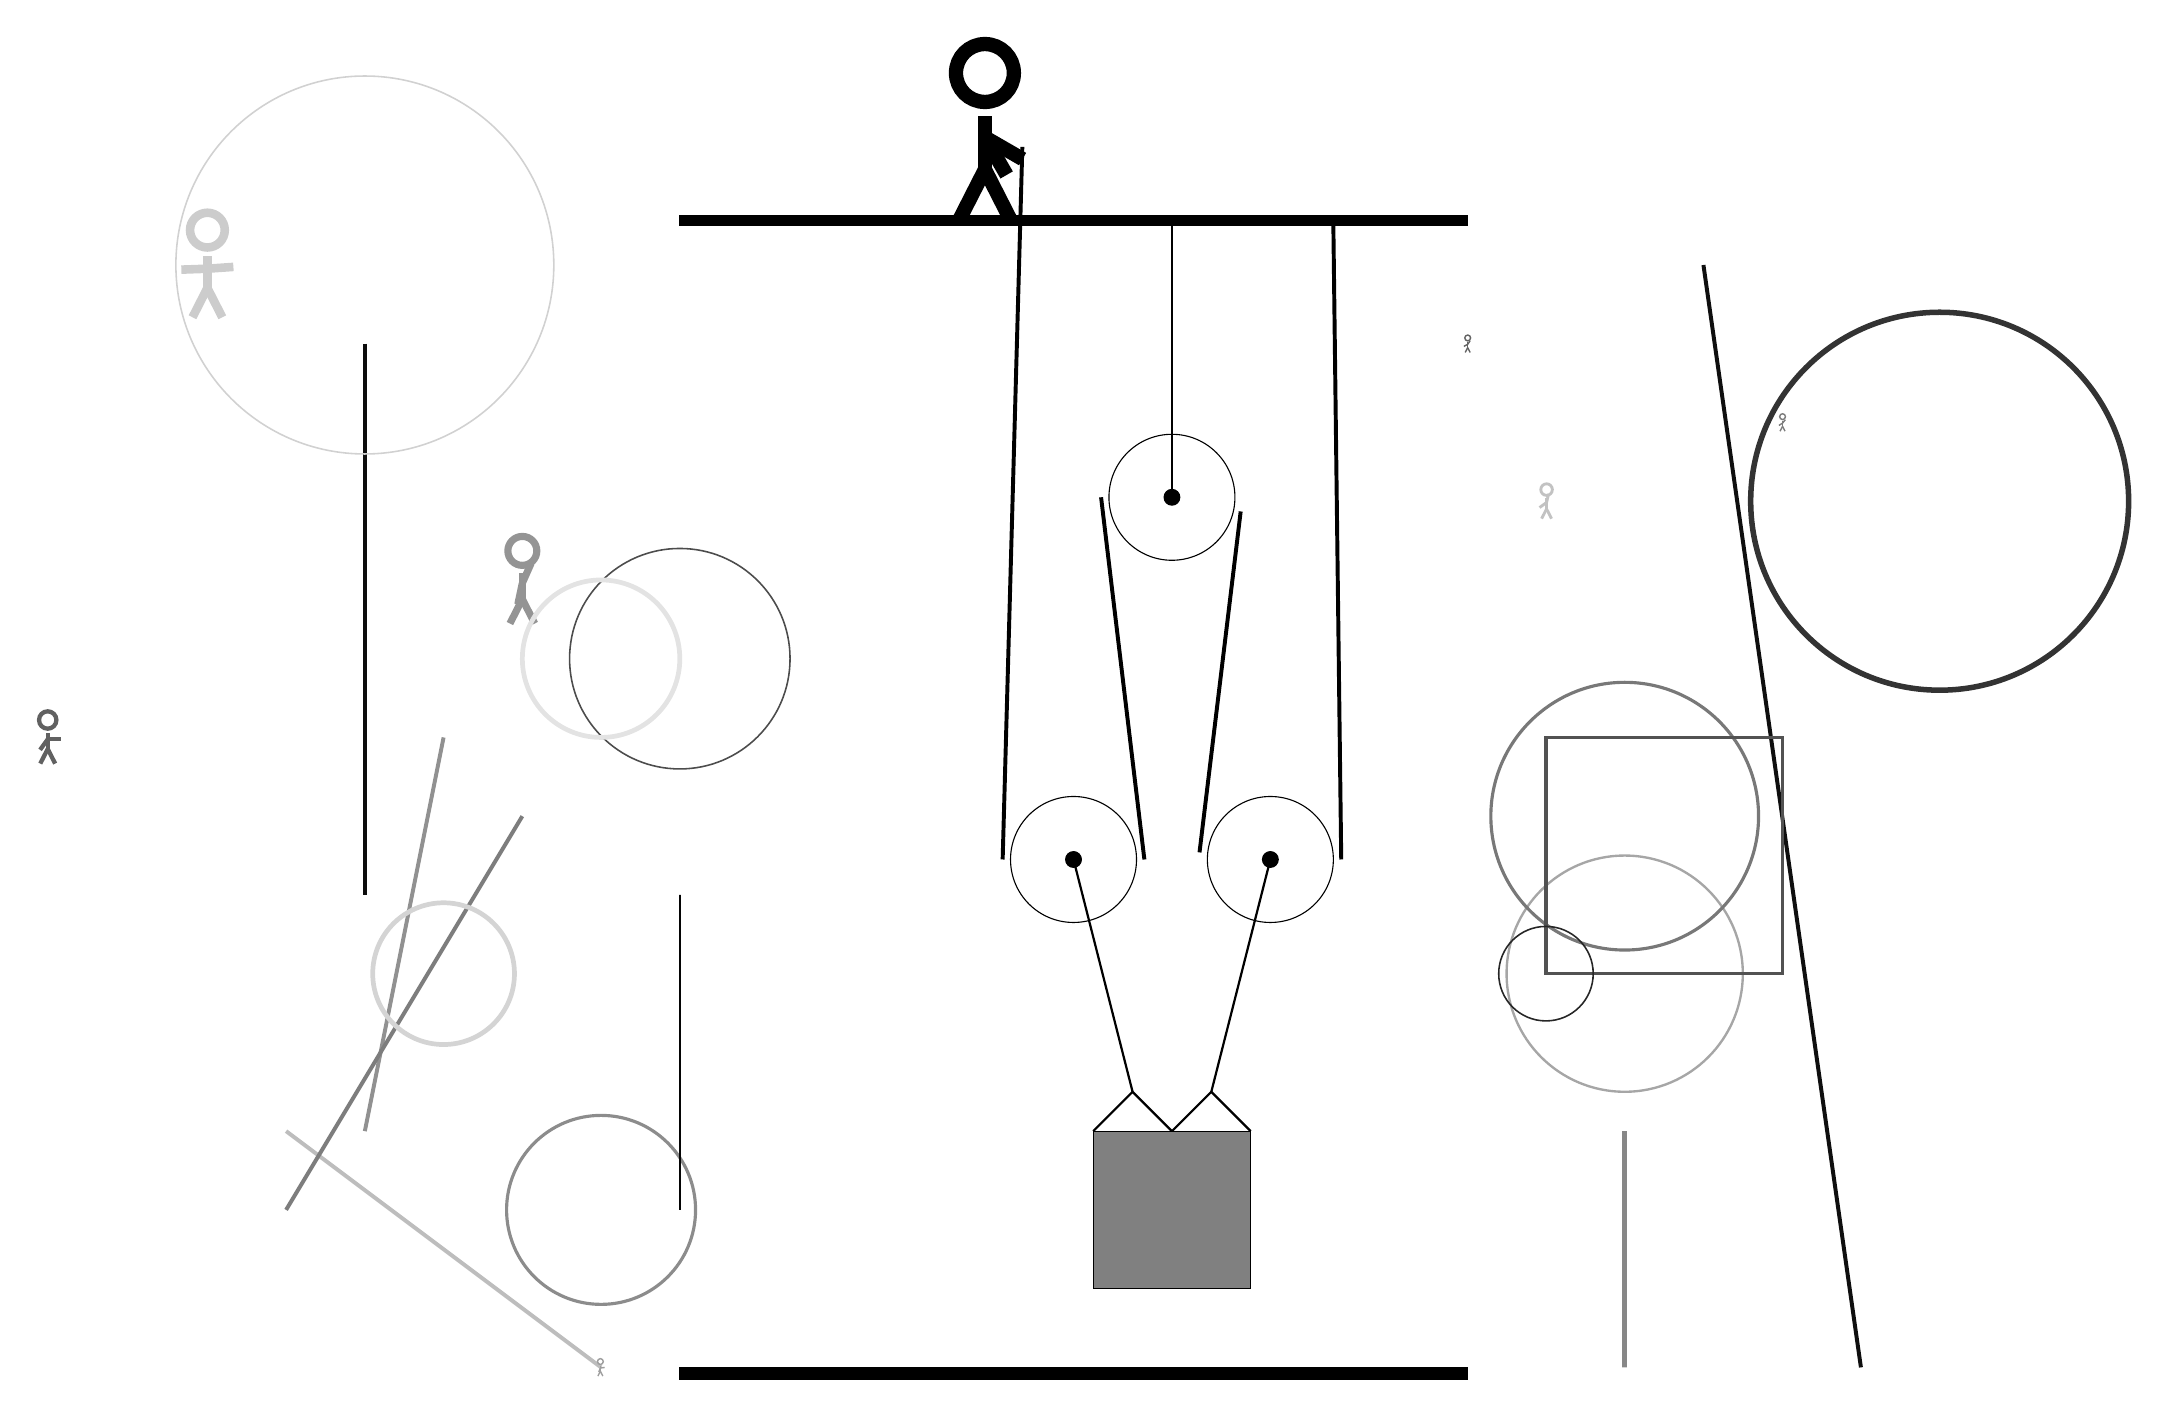
\begin{tikzpicture}
			%%%%% START %%%%%
			
			\draw[fill=black] (-4, 11.5) rectangle (6, 11.625);
			
			\draw (1, 3.45) circle (0.8);
			\draw[fill=black] (1, 3.45) circle (0.1);
			
			\draw (2.25, 8.05) circle (0.8);
			\draw[fill=black] (2.25, 8.05) circle (0.1);
			\draw[thick] (2.25, 8.05) -- (2.25, 11.5);
			
			\draw [line width=0.4mm, color=black!45](-5, -1) circle (1.2);
			
			\draw [line width=0.2mm, color=black!70](-4, 6) circle (1.4);
			\draw[line width=0.5mm, color=black!95](-8, 10) -- (-8, 3);
			\draw[line width=0.5mm, color=black!26](-9, 0) -- (-5, -3);
			\draw[line width=0.3mm, color=black!98] (-4, -1) rectangle (-4, 3);
			
			\node[line width=0.6mm, color=black!42] at (-6, 7) {\Strichmaxerl[5][78][66]};
			\draw[line width=0.5mm, color=black!94](9, 11) -- (11, -3);
			
			\draw [line width=0.3mm, color=black!35](8, 2) circle (1.5);
			\draw[line width=0.5mm, color=black!43](-7, 5) -- (-8, 0);
			
			\node[line width=0.2mm, color=black!61] at (6, 10) {\Strichmaxerl[1][28][56]};
			
			\draw [line width=0.6mm, color=black!11](-5, 6) circle (1.0);
			
			\node[line width=0.7mm, color=black!20] at (-10, 11) {\Strichmaxerl[6][2][4]};
			\draw [line width=0.4mm, color=black!53](8, 4) circle (1.7);
			
			\node[line width=0.2mm, color=black!24] at (7, 8) {\Strichmaxerl[2][36][77]};
			\draw[line width=0.7mm, color=black!47] (8, 0) rectangle (8, -3);
			\draw[line width=0.5mm, color=black!51](-9, -1) -- (-6, 4);
			\node[line width=0.5mm, color=black!62] at (-12, 5) {\Strichmaxerl[3][54][0]};
			\draw [line width=0.2mm, color=black!18](-8, 11) circle (2.4);
			\draw[line width=0.4mm, color=black!68] (7, 5) rectangle (10, 2);
			
			\draw [line width=0.7mm, color=black!80](12, 8) circle (2.4);
			\node[line width=0.4mm, color=black!38] at (-5, -3) {\Strichmaxerl[1][69][7]};
			
			\draw [line width=0.2mm, color=black!85](7, 2) circle (0.6);
			
			\draw [line width=0.6mm, color=black!17](-7, 2) circle (0.9);
			\node[line width=0.5mm, color=black!51] at (10, 9) {\Strichmaxerl[1][33][51]};
			
			\draw (3.5, 3.45) circle (0.8);
			\draw[fill=black] (3.5, 3.45) circle (0.1);
			
			\draw[thick] (3.5, 3.45) -- (2.75, 0.5);
			\draw[thick] (1, 3.45) -- (1.75, 0.5);
			\draw[thick]  (1.25, 0) -- (1.75, 0.5) -- (2.25, 0);
			\draw[thick]  (2.25, 0) -- (2.75, 0.5) -- (3.25, 0);
			\draw[fill=black!50] (1.25, 0) rectangle (3.25, -2);
			
			\draw[line width=0.5mm] (0.35, 12.5) --  (0.1, 3.45);
			\centerarc[line width=0.5mm](1, 3.45)(180:360:0.9);
			\draw[line width=0.5mm] (1.9, 3.45) -- (1.35, 8.05);
			\centerarc[line width=0.5mm](2.25, 8.05)(-20:180:0.9);
			\draw[line width=0.5mm](3.123, 7.87) -- (2.6, 3.54);
			\centerarc[line width=0.5mm](3.5, 3.45)(160:360:0.9);
			\draw[line width=0.5mm](4.4, 3.45) -- (4.3, 11.5);
			
			\node at (-0.07, 12.7) {\Strichmaxerl[10][120][-30]};
			
			\draw[fill=black] (-4, -3) rectangle (6, -3.15);
			
			%%%%% END %%%%%
		\end{tikzpicture}
	\end{figure}	
\end{document}